\documentclass[border=4pt]{standalone}
\usepackage{tikz}
\usetikzlibrary{arrows.meta, positioning, calc, shapes.geometric, backgrounds, fit}
\usepackage{pgfplots}
\pgfplotsset{compat=1.18}
\usepgfplotslibrary{fillbetween}
\definecolor{deepblue}{RGB}{10, 40, 90}
\definecolor{spaceblue}{RGB}{30, 80, 160}
\definecolor{lightgray}{RGB}{245, 245, 248}
\definecolor{accentgold}{RGB}{180, 140, 40}
\definecolor{earthgreen}{RGB}{40, 120, 80}
\definecolor{warnred}{RGB}{170, 40, 40}
\begin{document}
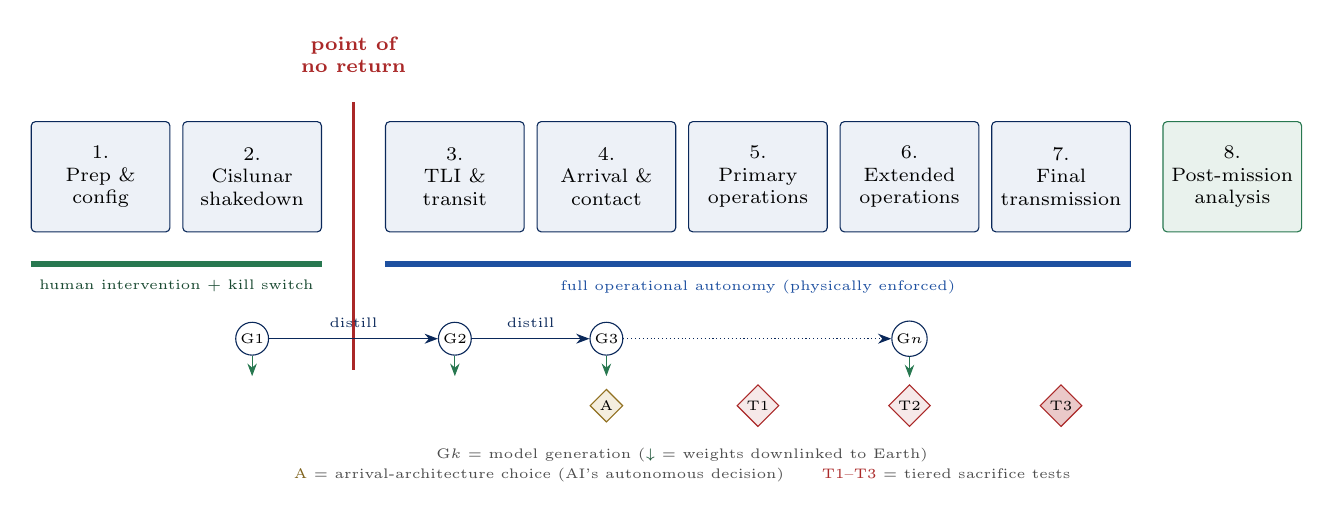
\begin{tikzpicture}[
  font=\footnotesize,
  phase/.style={draw=deepblue, fill=spaceblue!8, rounded corners=1.5pt, minimum height=14mm, align=center, inner sep=2pt, font=\scriptsize, text width=16.2mm},
]
\node[phase] (p1) at (0,0) {1.\\Prep \&\\config};
\node[phase, right=1.5mm of p1] (p2) {2.\\Cislunar\\shakedown};
\node[phase, right=8mm of p2] (p3) {3.\\TLI \&\\transit};
\node[phase, right=1.5mm of p3] (p4) {4.\\Arrival \&\\contact};
\node[phase, right=1.5mm of p4] (p5) {5.\\Primary\\operations};
\node[phase, right=1.5mm of p5] (p6) {6.\\Extended\\operations};
\node[phase, right=1.5mm of p6] (p7) {7.\\Final\\transmission};
\node[phase, right=4mm of p7, fill=earthgreen!10, draw=earthgreen] (p8) {8.\\Post-mission\\analysis};

% Point of no return: spans all tracks
\draw[warnred, line width=1.4pt] ($(p2.east)!0.5!(p3.west) + (0,-2.45)$) -- ($(p2.east)!0.5!(p3.west) + (0,0.95)$);
\node[font=\scriptsize\bfseries, color=warnred, align=center] at ($(p2.east)!0.5!(p3.west) + (0,1.55)$) {point of\\no return};

% Track 1: intervention / autonomy bars (uniform heights -> horizontal)
\draw[earthgreen, line width=2.2pt] ([yshift=-4mm]p1.south west) -- ([yshift=-4mm]p2.south east)
  node[midway, below=0.5mm, font=\tiny, color=earthgreen!60!black] {human intervention + kill switch};
\draw[spaceblue, line width=2.2pt] ([yshift=-4mm]p3.south west) -- ([yshift=-4mm]p7.south east)
  node[midway, below=0.5mm, font=\tiny, color=spaceblue] {full operational autonomy (physically enforced)};

% Track 2: generations with weights-downlink ticks
\node[circle, draw=deepblue, fill=white, inner sep=1pt, font=\tiny] (g1) at ([yshift=-13.5mm]p2.south) {G1};
\node[circle, draw=deepblue, fill=white, inner sep=1pt, font=\tiny] (g2) at ([yshift=-13.5mm]p3.south) {G2};
\node[circle, draw=deepblue, fill=white, inner sep=1pt, font=\tiny] (g3) at ([yshift=-13.5mm]p4.south) {G3};
\node[circle, draw=deepblue, fill=white, inner sep=1pt, font=\tiny] (gn) at ([yshift=-13.5mm]p6.south) {G$n$};
\draw[-{Stealth}, deepblue] (g1) -- (g2) node[midway, above=0.2mm, font=\tiny] {distill};
\draw[-{Stealth}, deepblue] (g2) -- (g3) node[midway, above=0.2mm, font=\tiny] {distill};
\draw[-{Stealth}, deepblue, densely dotted] (g3) -- (gn);
\foreach \g in {g1,g2,g3,gn}{\draw[-{Stealth[length=1.6mm]}, earthgreen, thin] (\g.south) -- ++(0,-2.6mm);}

% Track 3: decision points
\node[diamond, draw=accentgold!80!black, fill=accentgold!15, inner sep=0.9pt, font=\tiny] (da) at ([yshift=-22mm]p4.south) {A};
\node[diamond, draw=warnred, fill=warnred!10, inner sep=0.9pt, font=\tiny] (t1) at ([yshift=-22mm]p5.south) {T1};
\node[diamond, draw=warnred, fill=warnred!10, inner sep=0.9pt, font=\tiny] (t2) at ([yshift=-22mm]p6.south) {T2};
\node[diamond, draw=warnred, fill=warnred!25, inner sep=0.9pt, font=\tiny] (t3) at ([yshift=-22mm]p7.south) {T3};

% Single legend line
\node[font=\tiny, color=black!70, align=center] at ($(p4.south)!0.5!(p5.south) + (0,-2.95)$)
  {G$k$ = model generation ({\color{earthgreen!70!black}$\downarrow$} = weights downlinked to Earth)\\[0.4mm]
   {\color{accentgold!70!black}A} = arrival-architecture choice (AI's autonomous decision)\qquad
   {\color{warnred}T1--T3} = tiered sacrifice tests};
\end{tikzpicture}
\end{document}
